\documentclass[aspectratio=169,mathserif]{beamer}
\usepackage{pgfpages}
\usepackage{dsfont}
\usepackage{tikz}
\usetikzlibrary{calc}
\usetikzlibrary{graphs}
\usetikzlibrary{cd}
\usetikzlibrary{patterns}
\usetikzlibrary{backgrounds}
\usetikzlibrary{shapes}
\usetikzlibrary{decorations.pathmorphing}
\usetikzlibrary{decorations.pathreplacing}
%\usepackage{bussproofs}
\usepackage{ebproof}
\usepackage{stmaryrd}
\usepackage{colortbl}
\usepackage{booktabs}
\usepackage{listings}

% ACM palette {{{
\definecolor[named]{ACMBlue}{cmyk}{1,0.1,0,0.1}
\definecolor[named]{ACMYellow}{cmyk}{0,0.16,1,0}
\definecolor[named]{ACMOrange}{cmyk}{0,0.42,1,0.01}
\definecolor[named]{ACMRed}{cmyk}{0,0.90,0.86,0}
\definecolor[named]{ACMLightBlue}{cmyk}{0.49,0.01,0,0}
\definecolor[named]{ACMGreen}{cmyk}{0.20,0,1,0.19}
\definecolor[named]{ACMPurple}{cmyk}{0.55,1,0,0.15}
\definecolor[named]{ACMDarkBlue}{cmyk}{1,0.58,0,0.21}
%}}}

% Parameters {{{
\newcommand{\figsize}{\small}
\usecolortheme{rose}
\usecolortheme{seahorse}
%\usecolortheme{whale}
\setbeamercolor{structure}{fg=ACMBlue}
\setbeamercolor{example text}{fg=ACMOrange}
%\setbeameroption{show notes on second screen}
%\setbeamercolor{block title}{fg=black}

\setbeamertemplate{navigation symbols}{%
    \usebeamerfont{footline}%
    \usebeamercolor[fg]{footline}%
    \insertframenumber/\inserttotalframenumber
}

\AtBeginSection{\frame{\sectionpage}}

\lstset{basicstyle=\tt\scriptsize,language=C}

%}}}

% Macros {{{

% Some of the macros I defined trip up latexdiff,
% so I separate them in this file.
% vim: foldmethod=marker

% Notations
\newcommand{\kw}[1]{\ensuremath{ \mathsf{#1} }}
\newcommand{\ifr}[1]{\mathrel{[{#1}]}}
\newcommand{\que}{\circ}
\newcommand{\ans}{\bullet}
\newcommand{\vref}{\le_\kw{v}}
\newcommand{\mext}{\le_\kw{m}}
\newcommand{\refby}{\preceq}
\newcommand{\scref}{\sqsupseteq}
\newcommand{\screfd}{\sqsubseteq}
\newcommand{\unitset}{\mathds{1}}

% Multi-letter language interfaces
\newcommand{\li}[1]{\mathit{#1}}
% Calling conventions (language interface boundaries)
\newcommand{\cc}[2]{{ \kw{#1#2} }}

% Pointers for justified sequences %{{{

% Parameters
\newcommand{\pshift}{1.6ex}
\newcommand{\pcdist}{1}
\newcommand{\pcangle}{60}

% Pointer hook
\newcommand{\ph}[1]{%
  \tikz[remember picture]{\coordinate (#1);}}

% Pointer to
\newcommand{\ptc}[2]{%
  \tikz[remember picture,baseline,>={Latex[round,length=3.6pt]}]{
    \draw[->,#2]
      let \p{dest} = (#1),
          \n1 = {pow(veclen(\x{dest}, \y{dest}), 0.5) * 1.5},
          \p1 = ($(0,0)+(0,\pshift)$),
          \p4 = ($(\x{dest},0)+(0,\pshift)$),
          \p2 = ($(\p1)!\n1*\pcdist!-\pcangle:(\p4)$),
          \p3 = ($(\p4)!\n1*\pcdist!+\pcangle:(\p1)$) in
        (\p1) .. controls (\p2) and (\p3) .. node[pos=0.5] (top) {} (\p4);
    \pgfresetboundingbox
    \path[use as bounding box] (0,0 |- top);
}}
\newcommand{\pt}[1]{%
  \ptc{#1}{gray}}
\newcommand{\bpt}[1]{%
  \ptc{#1}{black,thick,>={Latex[round,length=4pt]}}}

% TikZ setup
\pgfdeclarelayer{tint}
\pgfdeclarelayer{nodes}
\pgfsetlayers{tint,background,main,nodes}
\selectcolormodel{cmyk}

% Parameters for diagrams
\newcommand{\stens}{0.6}

% The intensity of colors in figures and row highlighting respectively.
% These should be the same, otherwise they are just confusing to look at
% side by side, especially on a printout.
\newcommand{\filltint}{!35}
\newcommand{\tbltint}{\filltint}

% Colors used in the World transitions section
\newcommand{\colorA}{ACMDarkBlue}
\newcommand{\colorB}{ACMDarkBlue}
\newcommand{\internalA}[1]{\textcolor{\colorA}{#1}}
\newcommand{\internalB}[1]{\textcolor{\colorB}{#1}}

% Refinement tiles {{{

\newenvironment{tile}[1]{%
  \begin{tikzpicture}[baseline,yscale=0.36,xscale=0.5]
    \figsize
    \tikzset{to path={
      .. controls ($(\tikztostart)!\stens!(\tikztostart -| \tikztotarget)$)
              and ($(\tikztotarget)!\stens!(\tikztotarget -| \tikztostart)$) ..
      (\tikztotarget) \tikztonodes}}
    \tikzset{#1}
    % Coordinates for things on the left
    \coordinate (TL) at (-1,1);
    \coordinate (L) at (-1,0);
    \coordinate (BL) at (-1,-1);
    \coordinate (TLB) at (-0.3,1);
    \coordinate (BLB) at (-0.3,-1);
    % Coordinates for things on the right
    \coordinate (TR) at (1,1);
    \coordinate (R) at (1,0);
    \coordinate (BR) at (1,-1);
    \coordinate (TRB) at (0.3,1);
    \coordinate (BRB) at (0.3,-1);
    % Center node, for crossing
    \coordinate (T) at (0,+1.5);
    \node[circle,inner sep=2pt] (C) at (0,0) {};
    \coordinate (B) at (0,-1.5);
    % Computed coordinates
    \coordinate (TLC) at ($(T-|L)$);
    \coordinate (BLC) at ($(B-|L)$);
    \coordinate (TRC) at ($(T-|R)$);
    \coordinate (BRC) at ($(B-|R)$);
}{%
  \end{tikzpicture}
}
\newcommand{\simproof}[2]{%
  \begin{pgfonlayer}{nodes}
    \node[draw,rectangle,fill=white,rounded corners=2pt,minimum height=0.5cm,minimum width=0.8cm] at #1 {#2};
  \end{pgfonlayer}
}
\newcommand{\drawsc}{%
  \draw[thick,rounded corners=1mm]
}
\newcommand{\filltop}[1]{%
  \begin{pgfonlayer}{tint}
    \fill[#1] (TLC) rectangle (R);
  \end{pgfonlayer}
}
\newcommand{\fillbot}[1]{%
  \begin{pgfonlayer}{tint}
    \fill[#1] (L) rectangle (BRC);
  \end{pgfonlayer}
}
\newcommand{\fillboth}[1]}}



% adjust borders on this
\renewcommand{\simproof}[2]{%
  \begin{pgfonlayer}{nodes}
    \node[draw,rectangle,fill=white,rounded corners=2pt,
      minimum height=0.5cm,minimum width=0.8cm,inner sep=2pt] at #1 {#2};
  \end{pgfonlayer}
}
\renewcommand{\drawsc}{%
  \draw[thick,rounded corners=1mm]
}

\newcommand{\osimproof}[1]{\draw[fill=white] #1 circle[radius=2mm,aspect=1];}

%\renewcommand{\filltint}{!40}

\newcommand{\drawsb}[2]{%
  \draw (#1) -- node[pos=0.6] (sbT) {} +(-0.2ex,0) |- (#1 |- #2);
  \draw (sbT.center) -- (sbT.center |- #2);
  \draw (#1 -| #2) -- node[pos=0.6] (sbT) {} +(0.2ex,0) |- (#2);
  \draw (sbT.center) -- (sbT.center |- #2);
}

\newcommand{\cprog}[2]{
  \begin{scope}[every node/.style={align=left,inner sep=1ex}]
    \scriptsize \tt
    \node<#1> (C1) at (0,2) {
      int mult(n, p) \{ \\
      \:\: return n * p; \\
      \}
    };
    \node<#2> (C2) at (1,2) {
      int sqr(n) \{ \\
      \:\: return mult(n, n); \\
      \}
    };
    \node<#1> (C3) at (2,2) {
      int main() \{ \\
      \:\: return sqr(3); \\
      \}
    };
  \end{scope}
}

\newcommand{\sprog}[3]{
  \begin{scope}[every node/.style={align=left,inner sep=1ex}]
    \scriptsize \tt
    \setlength{\tabcolsep}{0.5ex}
    \node<#1> (#31) at (0,#2) {
      \begin{tabular}{rl}
        mult: & \%eax := \%ebx \\
              & \%eax *= \%ecx \\
              & ret
      \end{tabular}
    };
    \node<#1> (#32) at (1,#2) {
      \begin{tabular}{rl}
        sqr: & \%ecx := \%ebx \\
             & call mult \\
         L1: & ret
      \end{tabular}
    };
    \node<#1> (#33) at (2,#2) {
      \begin{tabular}{rl}
        main: & \%ebx := 3 \\
              & call sqr \\
          L2: & ret
      \end{tabular}
    };
  \end{scope}
}

% }}}

% TikZ pic's {{{

\tikzset{filesys/.pic={ %{{{
  \begin{scope}[xscale=0.33,yscale=0.5,yshift=0.5cm]
    \tiny
    \node[draw,circle] {\tt /}
      child {node {\tt bin}}
      child {node {\tt etc}}
      child[missing] { }
      child {node {\ldots}};
  \end{scope}
}}
%}}}

\tikzset{hdd/.pic={ %{{{
  \begin{scope}[xscale=0.75,yscale=0.25,yshift=-0.66cm]
    \draw[fill,shade,shading angle=90,left color=ACMGreen,right color=ACMGreen\filltint]
      (-1,1) arc[start angle=-180,end angle=0,radius=1] --
      (+1,0) arc[start angle=0,end angle=-180,radius=1] --
      cycle;
    \draw[fill=ACMGreen] (0,1) ellipse[radius=1];
    \draw (-1,0.33) arc[start angle=-180,end angle=0,radius=1];
    \draw (-1,0.66) arc[start angle=-180,end angle=0,radius=1];
  \end{scope}
}}
%}}}

\tikzset{cpu/.pic={ %{{{
  \begin{scope}[scale=0.4]
    \tikzset{every path/.style={
      decoration={
        border,
        angle=-90,
        segment length=1mm,
        amplitude=2mm,
        pre=moveto,
        pre length=2mm,
        %post=moveto,
        %post length=0.5mm
      }
    }}
    \draw[fill=ACMRed\filltint] (-1,-1) rectangle (+1,+1);
    \node {\scriptsize CPU};
    \draw[decorate] (-1,-1) -- (+1,-1);
    \draw[decorate] (+1,-1) -- (+1,+1);
    \draw[decorate] (+1,+1) -- (-1,+1);
    \draw[decorate] (-1,+1) -- (-1,-1);
    %\draw (+1,-1) -- (+1,+1);
     % -- (-1,+1) -- cycle;
  \end{scope}
}}
%}}}

\tikzset{nic/.pic={ %{{{
  \begin{scope}[xscale=0.15,yscale=0.2,xshift=-3.5cm,yshift=-2.5cm]
    \draw[fill=ACMGreen] (7,4) -| (0,1) -| (1,0) -| (4,1) -| (5,0) -| (6,1) -- (7,1);
    \draw[thick] (7,0) |- (8,5);
    \node at (3.5,2.5) {\scriptsize NIC};
    \tikzset{every path/.style={
      ACMYellow,
      thick,
      decoration={
        border,
        angle=90,
        segment length=0.5mm,
        amplitude=1.8mm
      }
    }}
    \draw[decorate] (1.33,0.1) -- (4,0.1);
    \draw[decorate] (5.33,0.1) -- (6,0.1);
  \end{scope}
}}
%}}}

\tikzset{l-nic/.pic={ %{{{
  \begin{scope}[xscale=-0.15,yscale=0.2,xshift=-3.5cm,yshift=-2.5cm]
    \draw[fill=ACMGreen] (7,4) -| (0,1) -| (1,0) -| (4,1) -| (5,0) -| (6,1) -- (7,1);
    \draw[thick] (7,0) |- (8,5);
    \node at (3.5,2.5) {\scriptsize NIC};
    \tikzset{every path/.style={
      ACMYellow,
      thick,
      decoration={
        border,
        angle=-90,
        segment length=0.5mm,
        amplitude=1.8mm
      }
    }}
    \draw[decorate] (1.33,0.1) -- (4,0.1);
    \draw[decorate] (5.33,0.1) -- (6,0.1);
    %\draw[decorate] (4, 0.1) -- (1.33,0.1);
    %\draw[decorate] (6, 0.1) -- (5.33,0.1);
  \end{scope}
}}
%}}}

\tikzset{eth/.pic={ %{{{
  \begin{scope}[scale=0.2,xscale=1.5,yshift=-5mm,xshift=-2cm]
    \draw[fill=ACMYellow\filltint]
      (0,0) rectangle (1,1);
    \draw[ACMYellow!80!black,decorate,decoration={
        border,angle=-90,segment length=0.25mm,amplitude=1.5mm}]
      (0.05,0.18) -- (0.05,1);
    \fill[ACMYellow] (1,2.5mm) rectangle (5,7.5mm);
    \draw (5,2.5mm) -- (1,2.5mm) (1,7.5mm) -- (5,7.5mm) -- cycle;
  \end{scope}
}}
%}}}

\tikzset{l-eth/.pic={ %{{{
  \begin{scope}[scale=-0.2,xscale=1.5,yshift=-5mm,xshift=-2cm]
    \draw[fill=ACMYellow\filltint]
      (0,0) rectangle (1,1);
    \draw[ACMYellow!80!black,decorate,decoration={
        border,angle=-90,segment length=0.25mm,amplitude=1.5mm}]
      (0.05,0.18) -- (0.05,1);
    \fill[ACMYellow] (1,2.5mm) rectangle (5,7.5mm);
    \draw (5,2.5mm) -- (1,2.5mm) (1,7.5mm) -- (5,7.5mm) -- cycle;
  \end{scope}
}}
%}}}

%}}}

% Front matter {{{
\title{CompCertO}
\subtitle{Compiling Certified Open C Components}
\author{Jérémie Koenig \and Zhong Shao}
\institute{Yale University}
\date{PLDI '21, June 20--25, 2021}
\titlegraphic{
  \begin{tile}{xscale=1.5}
    \simproof{(C)}{$\le$}
    \drawsc (L) -- (R);
    \draw (T) -- (B);
    \begin{pgfonlayer}{tint}
      \fill[ACMLightBlue\filltint] (TLC) rectangle (C.center);
      \fill[ACMOrange\filltint] (L) rectangle (B);
      \fill[ACMBlue\filltint] (T) rectangle (R);
      \fill[ACMRed\filltint] (C.center) rectangle (BRC);
    \end{pgfonlayer}
  \end{tile}
}
%}}}

\begin{document}

\maketitle

\begin{frame}{Introduction} %{{{
  \note{In our shorter video,}
  \note[item]{Overview of CompCertO,}
  \note[item]{Equips CompCert with fully compositional correctness theorem}
  \note[item]{talked about how it fits in with existing and future research}

  CompCertO takes inspiration from game semantics
  and certified abstraction layers \\
  to provide a \textbf{fully compositional} version
  of CompCert's correctness proof.

  \pause\vfill
  \begin{center}
    \textbf{Key insight:} \\
    \Large
    Compositional compiler correctness is facilitated \\ by
    a \textbf{first-class} treatment of \textbf{calling conventions}.
  \end{center}
  \note[item]<2->{
    Often assumed that compositional semantics are too intricate to use
    for real-world compiler correctness, \\
    Our work shows, we can keep things from getting too hairy
    by a careful treatment of calling conventions}

  \vfill
  Using a form of \textbf{two-dimensional typing} 
  for transition systems and simulation proofs,
  we demonstrate that
  the use of \textbf{compositional semantics} for compiler correctness \\
  is tractable,
  challenging common wisdom and opening new avenues for future research.
\end{frame}
%}}}

\begin{frame}{Overview}
  \note{In this longer video,
    present our techniques in more detail.}
  \note[item]{Semantic model}
  \note[item]{Proof techniques used to derive comp corr}

  \tableofcontents
\end{frame}

\section{Whole-Program Semantics in CompCert}
\note{How semantics work in the original CompCert}

\begin{frame}[fragile]{Program semantics are given as transition systems} %{{{
  \begin{definition}
  A \textbf{transition system}
  $
    L = \langle S, {\rightarrow}, I, F \rangle
  $
  describes:
  \begin{itemize}
    \item State transitions ${\rightarrow} \subseteq S \times S$
    \item Initial states $I \subseteq S$
    \item Final states $F \subseteq S \times \kw{int}$
  \end{itemize}
  \end{definition}
  \note{CompCert uses transition systems to characterize behaviors of its
source and target programs}
  \note[item]{Set of states equipped with transition relation}
  \note[item]{Initial states specify how execution starts}
  \note[item]{Ultimately, final states provide an exit status
    for the program}

  \begin{example}
  \[
    \left\llbracket
    \begin{tabular}{c}
      \begin{lstlisting}
int main(void) {
  return 21 * 2;
}
      \end{lstlisting}
    \end{tabular}
    \right\rrbracket : \quad
    I \ni
    s \rightarrow
    s' \rightarrow
    \cdots \rightarrow
    s^n \mathrel{F}
    42
  \]
  \end{example}
\end{frame}
%}}}

\begin{frame}[fragile]{Refinement is established using forward simulations} %{{{
  \note{To show compilation preserves semantics,
    need to relate behaviors the source and target program.}

  \pause
  \begin{definition}
    A \textbf{forward simulation} $L_1 \le L_2$
    %$L_1 = \langle S_1, {\rightarrow}_1, I_1, F_1 \rangle$ to
    %$L_2 = \langle S_2, {\rightarrow}_2, I_2, F_2 \rangle$ \\
    is a relation $R \subseteq S_1 \times S_2$ such that:
    \\[1em]
    \centering
      \begin{tikzcd}
        * \ar[d, dash, double] \ar[r, "I_1", dash] & s_1 \ar[d, dash, dashed, "R"] &
        s_1 \ar[r] \ar[d, dash, "R"'] & \!\! {}_1 \:\, s_1' \ar[d, dash, dashed, "R"] &
        s_1 \ar[r, dash, "F_1"] \ar[d, dash, "R"'] & v \ar[d, double, dash]
        \\
        * \ar[r, "I_2"', dash, dashed] & s_2 &
        s_2 \ar[r, dashed] & \!\! {}_2^* \:\, s_2' &
        s_2 \ar[r, dash, dashed, "F_2"'] & v
      \end{tikzcd}
  \end{definition}
  \note[item]<2->{CompCert uses forward simulations.}
  \note[item]<2->{Relation between source and target states}
  \note[item]<2->{For initial state in source, related initial state in targ}
  \note[item]<2->{Internal steps must preserve:
    step in source matched by sequence of steps in target}
  \note[item]<2->{If two states related and source is final,
    target final with same result}

  \note[item]<2->{If we have a source execution,
    iterate the step simulation property between initial and final state
    to show that the target program behaves in the same way.}
  \begin{example}%
    \centering
    \begin{tikzcd}[column sep=-2ex, row sep=4ex]
      \left\llbracket
      \begin{tabular}{c}
        \begin{lstlisting}
int main() { return 21*2; }
        \end{lstlisting}
      \end{tabular}
      \right\rrbracket : \quad {}
      \ar[d]
      & I_1 \ni {}
      & s_1 \ar[d, dash, "R"'] & {} \rightarrow
      s_1' \rightarrow
      \cdots \rightarrow {}
      & s_1^n \ar[d, dash, "R", dashed] & {} \mathrel{F_1}
      4 2
      \\
      \left\llbracket
      \begin{tabular}{c}
        \begin{lstlisting}
int main() { return  42;  }
        \end{lstlisting}
      \end{tabular}
      \right\rrbracket : \quad {}
      & I_2 \ni {}
      & s_2 & {} \rightarrow
      s_2' \rightarrow
      \cdots \rightarrow {}
      & s_2^p & {} \mathrel{F_2}
      42
    \end{tikzcd}
  \end{example}

\end{frame}
%}}}

\begin{frame}[fragile]{Forward simulations are transitive} %{{{
  \note{Key property of simulations: they are transitive}
  \note[item]{If we have sim from $L_1$ to $L_2$ and $L_2$ to $L_3$,
    diagrams can be pasted, meaning that}
  \note[item]<2->{if compose the two sim rel,
    obtain a sim rel again.}
  \note[item]<2->{this vertical compositionality
    is what makes verif compcert possible: \\ verif passes one by one}

  If $L_1 \le L_2$ and $L_2 \le L_3$, the diagrams can be pasted vertically:
  \[
    \begin{tikzcd}[column sep=3em]
      L_1 : &
      * \ar[r, "I_1", dash]
        \only<1>{\ar[d, dash, double]}
        \only<2->{\ar[dd, dash, double]}
      &
      s_1
        \only<1>{\ar[d, dash, dashed, "R"]}
        \only<2->{\ar[dd, dash, dashed, "R \cdot S"]}
      &
      s_1 \ar[r]
        \only<1>{\ar[d, dash, "R"']}
        \only<2->{\ar[dd, dash, "R \cdot S"']}
      &
      \!\! {}_1 \:\, s_1'
        \only<1>{\ar[d, dash, dashed, "R"]}
        \only<2->{\ar[dd, dash, dashed, "R \cdot S"]}
      &
      s_1 \ar[r, dash, "F_1"]
        \only<1>{\ar[d, dash, "R"']}
        \only<2->{\ar[dd, dash, "R \cdot S"']}
      &
      v
        \only<1>{\ar[d, double, dash]}
        \only<2->{\ar[dd, double, dash]}
      \\
      \only<1>{
        L_2 : &
        * \ar[d, dash, double] \ar[r, "I_2", dash, dashed] &
        s_2 \ar[d, dash, dashed, "S"] &
        s_2 \ar[r, dashed] \ar[d, dash, "S"'] &
        \!\! {}^*_2 \:\, s_2' \ar[d, dash, dashed, "S"] &
        s_2 \ar[r, dash, dashed, "F_2"] \ar[d, dash, "S"'] &
        v \ar[d, double, dash]
      }
      \only<2->{
        & & & & \textcolor{white}{s_2'}
      }
      \\
      L_3 : &
      * \ar[r, "I_3", dash, dashed] &
      s_3 &
      s_3 \ar[r, dashed] &
      \!\! {}_3^* \:\, s_3' &
      s_3 \ar[r, dash, dashed, "F_3"] &
      v
    \end{tikzcd}
  \]
  \pause
  \[
    s_1 \mathrel{[R \cdot S]} s_3 \: \Leftrightarrow \:
    \exists s_2 \mathrel{.}
      s_1 \mathrel{R} s_2 \, \wedge \, s_2 \mathrel{S} s_3
  \]

  \vfill
  This enables vertical composition of proofs for successive compilation passes.
\end{frame}
%}}}

\section{Open Semantics in CompCertO}
\note{That's how it works in CompCert \\
  In CompCertO, generalize to take into account
  interactions between prog comp}

\begin{frame}{Cross-component calls are described by language interfaces} %{{{
  \note{Starting point: notion of language interface \\ }
  \begin{definition}
    A \textbf{language interface} $A = \langle A^\que, A^\ans \rangle$ provides:
    \begin{itemize}
      \item a set $A^\que$ of \textbf{questions}
      \item a set $A^\ans$ of \textbf{answers}
    \end{itemize}
  \end{definition}

  \pause
  \note<2->{at C level: questions = function call (which, arguments), \\
    when returns, gives answer (its return value) \\}
  \begin{example}
    I will use $\mathcal{C}$ % = \langle \mathcal{C}^\que, \mathcal{C}^\ans \rangle$
    as a (simplified) interface for the C language:
    \begin{itemize}
      \item \makebox[14em][l]{Questions are \textbf{function calls}}
        $\mathcal{C}^\que :=
        \{ f(\vec{v}) \mid f \in \kw{ident}, \vec{v} \in \kw{val}^* \}$
      \item \makebox[14em][l]{Answers are \textbf{return values}}
        $\mathcal{C}^\ans := \kw{val}$
        %\{ v \mid v \in \kw{val} \}$
    \end{itemize}
    \pause
  \note<3->{At assembly level, more involved \\
    Question = answer = machine state \\
    Contents of registers, stack of pending return addresses}
    For assembly,
    $\mathcal{A}$ % = \langle \mathcal{A}^\que, \mathcal{A}^\ans \rangle$ 
    uses registers $R = \{ \kw{eax}, \kw{ebx}, \kw{ecx}, \kw{pc} \}$
    and a \emph{stack} of return addresses:
    \begin{itemize}
      \item \makebox[14em][l]{Questions are \textbf{machine states}}
        $\mathcal{A}^\que =
         \kw{val}^R \times \kw{val}^*$
      \item \makebox[14em][l]{Answers are the same thing}
        $\mathcal{A}^\ans =
         \kw{val}^R \times \kw{val}^*$
    \end{itemize}
  \end{example}
\end{frame}
%}}}

\begin{frame}[fragile]{Incoming calls generalize initial/final-state predicates} %{{{
  \note{To take into account \emph{incoming} calls, \\
    update transition systems with language interface parameter $B$.}
  \note[item]{Initial states now index by questions of $B$}
  \note[item]{Final states produce answers of $B$}

  \begin{definition}[Adding incoming calls]
  A \textbf{transition system}
  $
    L : B %= \langle S, {\rightarrow}, I, F \rangle
  $
  for a language interface $B = \langle B^\que, B^\ans \rangle$ has:
  \begin{itemize}
    \item State transitions ${\rightarrow} \subseteq S \times S$
    \item Initial states $I \subseteq B^\que \times S$
    \item Final states $F \subseteq S \times B^\ans$
  \end{itemize}
  \end{definition}
  \pause
  \note[item]<2->{
    Creates difficulty:
    how do source and target interactions relate?
  }
  \note[item]<2->{Calling conventions can be complex; looking at
    questions in the example}
  \note[item]<2->{Program counter must point to the code for mult,}
  \note[item]<2->{registers ebx, ecx must store arguments}
  \note[item]<2->{There is also the stack of pending return addresses}
  \note[item]<2->{In the answer, top address popped from stack, used as
    the new pc}
  \note[item]<2->{Means that questions and answers not related
independently, \\
    instead, will need to formalize a 4-way relationship between
    source and target questions and answers}
  \begin{example}
    \vspace{0.5ex}
    \centering
    $\begin{array}{r@{{} : {}}c@{\qquad}c@{}c@{}c}
      %
      \left\llbracket
      \begin{tabular}{c}
        \begin{lstlisting}
int mult(x, y) {
  return x * y;
}
        \end{lstlisting}%
      \end{tabular}
      \right\rrbracket
      &
      \mathcal{C}
      &
      \kw{mult}(3, 4)
      &
      {} \mathrel{I_1}
      s_1 \rightarrow
      s_1' \rightarrow
      \cdots \rightarrow
      s_1^n \mathrel{F_1} {}
      &
      12
    \vspace{1em}
    \\
      \left\llbracket
      \begin{tabular}{c}
        \begin{lstlisting}
mult: eax := ebx
      eax *= ecx
      ret
        \end{lstlisting}%
      \end{tabular}
      \right\rrbracket
      &
      \mathcal{A}
      &
      \left[
     {\tiny
      \begin{array}{l@{{} \mapsto {}}r}
        \kw{pc}  & \kw{mult} \\
        \kw{eax} & 27 \\
        \kw{ebx} & \mathbf{3} \\
        \kw{ecx} & \mathbf{4} \\
        \multicolumn{2}{r}{\textit{stack: } x \vec{k}}
      \end{array}}
      \right]
      &{} \mathrel{I_2}
      s_2 \rightarrow
      s_2' \rightarrow
      \cdots \rightarrow
      s_2^p \mathrel{F_2} {}&
      \left[
     {\tiny
      \begin{array}{l@{{} \mapsto {}}r}
        \kw{pc}  & x \\
        \kw{eax} & \mathbf{12} \\
        \kw{ebx} & 3 \\
        \kw{ecx} & 4 \\
        \multicolumn{2}{r}{\textit{stack: } \vec{k}}
      \end{array}}
      \right]
    \end{array}$
  \end{example}
\end{frame}
%}}}

\begin{frame}{First-class Calling Conventions} %{{{
  \note{To deal with this,
    our notion of simulation convention
    uses a set of worlds.}
  \note[item]{Worlds ensure that questions and answers are related
    consistently}
  \begin{definition}
    A \textbf{simulation convention} $\mathbb{R} : A_1 \Leftrightarrow A_2$
    provides:
    \begin{itemize}
      \item A set $W$ of \textbf{worlds}
      \item A relation
        $\mathbb{R}^\que \subseteq W \times A_1^\que \times A_2^\que$
        between the questions of $A_1$ and $A_2$
      \item A relation
        $\mathbb{R}^\ans \subseteq W \times A_1^\ans \times A_2^\ans$
        between the answers of $A_1$ and $A_2$
    \end{itemize}
  \end{definition}
  %Questions and their corresponding answers must be related at the same world.
  \pause
  \note[item]<2->{In our example, use the stack as world}
  \begin{example}
    The convention
    $\mathbb{C} : \mathcal{C} \Leftrightarrow \mathcal{A}$
    uses the \emph{return stacks} as worlds, \pause and the relations:
    \[
      \note[item]<3->{Relation on questions explains
         how function and arguments encoded,
         constrains world to be the same stack used in question}
      \begin{prooftree}
        \hypo{\mathit{rs}[\kw{pc}] = f}
        \hypo{\vec{v} \sqsubseteq \mathit{rs}[\kw{ebx}, \kw{ecx}]}
        \infer2{x \vec{k} \Vdash
          f(\vec{v})
          \mathrel{\mathbb{C}^\que}
          (\mathit{rs}, x \vec{k})}
      \end{prooftree}
      \qquad
      \pause
      \note[item]<4->{Then in answer, use this information
        to formalize the return mechanism}
      \begin{prooftree}
        \hypo{\mathit{rs}[\kw{eax}] = v'}
        \hypo{\mathit{rs}[\kw{pc}] = x}
        \infer2{x \vec{k} \Vdash
          v'
          \mathrel{\mathbb{C}^\ans}
          (\mathit{rs},\vec{k})}
       \end{prooftree}
    \]
  \end{example}
  \pause
  \note[item]<5->{Using this notion of simulation conventions,
    can update the definition of forward simulations.}
\end{frame}
%}}}

\begin{frame}[fragile]{Simulations modulo conventions} %{{{
  \note{Main change is that sim is indexed by sim conv, \\
    relation is indexed by a world of sim conv. \\
    Then generalized the simulation properties for initial, final states \\
    to take questions, answers into account.}
  \note[item]{World is threaded through the simulation}
  \note[item]{Sim rel can maintain invariants so that ultimate answers
    related at the right world}
  \note[item]{To summarize,
    extended CompCert semantics using language interfaces, \\
    so that prog comp invoked with arbitrary questions, \\
    and we used
    simulation conventions formalize abstraction gap bw src, tgt}
  \note[item]{Now, must go one step futher, allow components
    to make outgoing external calls.}

  %Consider
  %$\mathbb{R} = \langle W, \mathbb{R}^\que, \mathbb{R}^\ans \rangle : B_1 \Leftrightarrow B_2$
  %and two transition systems $L_1 : B_1$ and $L_2 : B_2$.

  \begin{definition}[Adding simulation conventions]
    A \textbf{forward simulation} $L_1 \le_\mathbb{R} L_2$
    is a relation $R \subseteq W \times S_1 \times S_2$ such that:
    \\[1ex]
    \centering
      \begin{tikzcd}
        q_1 \ar[d, dash, "w \Vdash \mathbb{R}^\que"'] \ar[r, "I_1", dash] &
        s_1 \ar[d, dash, dashed, "w \Vdash R"] & &
        s_1 \ar[r] \ar[d, dash, "w \Vdash R"'] &
        \!\! {}_1 \:\, s_1' \ar[d, dash, dashed, "w \Vdash R"] & &
        s_1 \ar[r, dash, "F_1"] \ar[d, dash, "w \Vdash R"'] &
        r_1 \ar[d, dash, dashed, "w \Vdash \mathbb{R}^\ans"]
        \\
        q_2 \ar[r, "I_2"', dash, dashed] & s_2 & &
        s_2 \ar[r, dashed] & \!\! {}_2^* \:\, s_2' & &
        s_2 \ar[r, dash, dashed, "F_2"'] & r_2
      \end{tikzcd}
  \end{definition}
  \begin{example}%
    \centering
    \begin{tikzcd}[column sep=-2ex, row sep=4ex]
      \left\llbracket
      \begin{tabular}{c}
        \begin{lstlisting}
int mult(x, y) { ... }
        \end{lstlisting}
      \end{tabular}
      \right\rrbracket : \quad
      \ar[d, draw opacity=0, "\le_{\mathbb{C}}"']
      & \kw{mult}(3, 4) \ar[rr, dash, "I_1"]
        \ar[d, dash, "x\vec{k} \Vdash \mathbb{C}^\que"'] & \qquad
      & s_1 \ar[d, dash, "x\vec{k} \Vdash R"', dashed] & {} \rightarrow
      s_1' \rightarrow
      \cdots \rightarrow {}
      & s_1^n \ar[d, dash, "x\vec{k} \Vdash R", dash] \ar[rr, dash, "F_1"] & \qquad &
      42 \ar[d, dash, dashed, "x\vec{k} \Vdash \mathbb{C}^\ans"]
      \\
      \left\llbracket
      \begin{tabular}{c}
        \begin{lstlisting}
mult: %eax := %ebx ...
        \end{lstlisting}
      \end{tabular}
      \right\rrbracket : \quad
      & {[\equiv]} \ar[rr, dash, "I_2"', dashed] & \qquad
      & s_2 & {} \rightarrow
      s_2' \rightarrow
      \cdots \rightarrow {}
      & s_2^p \ar[rr, "F_2"', dash, dashed] & \qquad \quad &
      {[\equiv]}
    \end{tikzcd}
  \end{example}
\end{frame}
%}}}

\begin{frame}[fragile]{Outgoing calls use their own predicates} %{{{
  \note{In third and final iteration, \\
    transition systems \emph{use} language interface $A$ for their outgoing calls, \\
    to \emph{provide} a language interface $B$ for their incoming calls.}
  \note[item]{Two new state predicates:}
  \note[item]{The relation $X$ identifies \emph{external states}
    and their associated question in $A$}
  \note[item]{The relation $Y$ explains how external state
    is updated once we get the answer}

  \begin{definition}[Adding outgoing calls]
  A \textbf{transition system}
  $
    L : A \twoheadrightarrow B
  $
  is a tuple
  $L = \langle S, {\rightarrow}, I, X, Y, F \rangle$
  where
  \begin{itemize}
    \item the components $S$, $\rightarrow$, $I$, $F$ are as before,
    \item $X \subseteq S \times A^\que$
      identifies \textbf{external states},
    \item $Y \subseteq S \times A^\ans \times S$
      identifies \textbf{resumption states}.
  \end{itemize}
  We will use the infix notation $s \mathrel{X} q \leadsto r \mathrel{Y^s} s'$.
  \end{definition}
  \pause
  \note[item]<2->{Example: as before, execution initiated by an incoming call
    (to square function)}
  \note[item]<2->{As some point, reach external state $s_i$}
  \note[item]<2->{Triggers an external call to mult}
  \note[item]<2->{When we get answer, use return value to update $s_i$,
    resume execution in state $s_i'$}
  \note[item]<2->{Eventually reach final state $s_n$,
    produce answer $9$ to original question sqr(3)}
  \begin{example}
    \begin{center} $
    \begin{array}{c}
      \left\llbracket
      \begin{tabular}{c}
        \begin{lstlisting}
int sqr(int x) {
  return mult(x, x);
}
        \end{lstlisting}%
      \end{tabular}
      \right\rrbracket \: : \:
      \mathcal{C} \twoheadrightarrow \mathcal{C}
    \vspace{1em} \\
      \kw{sqr}(3) \mathrel{I} s_0 \rightarrow \cdots \rightarrow
      s_i \mathrel{X}
      \kw{mult}(3,3) \leadsto 9
      \mathrel{Y^{s_i}} s_i' \rightarrow \cdots \rightarrow
      s_n \mathrel{F} 9
    \end{array}
    $ \end{center}
  \end{example}
\end{frame}
%}}}

\begin{frame}[fragile]{Simulations with Outgoing Calls} %{{{
  \note{Just need to extend simulation with a property for new predicates}
  \note[item]{Now, two indep sim conv for outgoing and incoming calls}
  \note[item]{For each outgoing question, simulation can choose world $w_A$
    of outgoing sim conv $\mathbb{R}_A$ and must show questions related
      at that world}
  \note[item]{Answers for these outgoing questions guaranteed to be related
    at that world, must reestablish simulation relation}
  \note[item]{This world independent from the world $w_B$ used for
    incoming question and the simulation relation.}
  \note[item]{In the example, use our calling convention
    for both incoming and outgoing calls,
    but call to mult uses a different world,
    where return label L has been added to stack.}
  \begin{definition}[Adding outgoing calls]
    A \textbf{forward simulation}
    $L_1 \le_{\mathbb{R}_A \twoheadrightarrow \mathbb{R}_B} L_2$
    is as before, with the following addition:
    \\[1ex]
    \centering
      \begin{tikzcd}
        s_1 \ar[r, "X_1", dash] \ar[d, "w_B \Vdash R"', dash] &
        m_1 \ar[rrr, dotted, dash] \ar[d, "w_A \Vdash \mathbb{R}_A^\que", dash, dashed] &&&
        n_1 \ar[r, "Y_1^{s_1}", dash] \ar[d, "w_A \Vdash \mathbb{R}_A^\ans"', dash] &
        s_1' \ar[d, "w_B \Vdash R", dash, dashed]
        \\
        s_2 \ar[r, "X_2"', dash, dashed] &
        m_2 \ar[rrr, dotted, dash] &&&
        n_2 \ar[r, "Y_2^{s_2}"', dash, dashed] &
        s_2'
      \end{tikzcd}
  \end{definition}
  \begin{example}
    \centering
    \begin{tikzcd}[column sep=0, row sep=4ex]
      \left\llbracket
      \begin{tabular}{c}
        \begin{lstlisting}
int sqr(x) { ... }
        \end{lstlisting}
      \end{tabular}
      \right\rrbracket :
      \ar[d, draw opacity=0, "\le_{ \mathbb{C} \rightarrow \mathbb{C} }"']
      &
      \cdots \rightarrow \hspace{-1.5ex} &
      s_1 \ar[d, dash, "x\vec{k} \Vdash R"'] &
      X_1 &
      \kw{mult}(3, 3) \ar[d, dash, dashed, "\mathsf{L}x\vec{k} \Vdash \mathbb{C}^\que"']
        \ar[rr, dotted, dash] & \quad \quad &
      9 \ar[d, dash, "\mathsf{L}x\vec{k} \Vdash \mathbb{C}^\ans"'] &
      Y_1^{s_1} &
      s_1' \ar[d, dash, dashed, "x\vec{k} \Vdash R"] &
      \hspace{-1.5ex} \rightarrow \cdots
      \\
      \left\llbracket
      \begin{tabular}{c}
%sqr: %ecx:=%ebx ..
        \begin{lstlisting}
.. call mult  L:..
        \end{lstlisting}
      \end{tabular}
      \right\rrbracket :
      &
      \cdots \rightarrow \hspace{-1.5ex} &
      s_2 &
      X_2 &
      {[\equiv]} \ar[rr, dotted, dash] & \quad &
      {[\equiv]} &
      Y_2^{s_2} &
      s_2' &
      \hspace{-1.5ex} \rightarrow \cdots
    \end{tikzcd}
  \end{example}
\end{frame}
%}}}

\begin{frame}{Summary} %{{{
  \note{To sum up:}
  \note[item]{Start from notion of language interface}
  \note[item]{Transition systems are parametrized by
    incoming and outgoing language interfaces}
  \note[item]{Simulation conventions are parametrized by
    source and target language interfaces}
  \note[item]{When two transition systems and two simulation conv
    have compatible types,
    can use them to formulate simulation property}
  %\centering
  \small
  \begin{tabular}{crcc}
    Language interface
  &
    \begin{tile}{scale=1.5}
      \fillboth{ACMLightBlue\filltint}
      \node {$A$};
    \end{tile}
  &
    \begin{tile}{scale=1.5}
      \fillleft{ACMLightBlue\filltint}
      \fillright{ACMBlue\filltint}
      \draw (T) node[above,overlay]{$L$} -- (B);
      \node[right,outer sep=0.8ex] at (L) {$A$};
      \node[left,outer sep=0.8ex] at (R) {$B$};
    \end{tile}
  &
    \begin{tabular}{c}
      Transition system \\
      $L : A \twoheadrightarrow B$
    \end{tabular}
  \vspace{1em} \\
    \begin{tabular}{c}
      Simulation convention \\
      $\mathbb{R} : A_1 \Leftrightarrow A_2$
    \end{tabular}
  &
    \begin{tile}{scale=1.5}
      \filltop{ACMLightBlue\filltint}
      \fillbot{ACMOrange\filltint}
      \drawsc (L) node[left] {$\mathbb{R}$} -- (R);
      \node[below,outer sep=1ex] at (T) {$A_1$};
      \node[above,outer sep=1ex] at (B) {$A_2$};
    \end{tile}
  &
    \begin{tile}{scale=1.5}
      \simproof{(C)}{$\le$}
      \drawsc (L) node[left] {$\mathbb{R}_A$}
        -- (R) node[right] {$\mathbb{R}_B$};
      \draw (T) node[above] {$L_1$} -- (B) node[below] {$L_2$};
      \begin{scope}[every node/.style={outer sep=0.3ex}]
        \node[below right] at (TLC) {$A_1$};
        \node[below left] at (TRC) {$B_1$};
        \node[above right] at (BLC) {$A_2$};
        \node[above left] at (BRC) {$B_2$};
      \end{scope}
      \begin{pgfonlayer}{tint}
        \fill[ACMLightBlue\filltint] (TLC) rectangle (C.center);
        \fill[ACMOrange\filltint] (L) rectangle (B);
        \fill[ACMBlue\filltint] (T) rectangle (R);
        \fill[ACMRed\filltint] (C.center) rectangle (BRC);
      \end{pgfonlayer}
    \end{tile}
  &
    \begin{tabular}{c}
      Forward simulation \\
      $L_1 \le_{\mathbb{R}_A \twoheadrightarrow \mathbb{R}_B} L_2$
    \end{tabular}
  \end{tabular}
\end{frame}
%}}}

\section{Building simulation proofs}

\begin{frame}[fragile]{Horizontal and Vertical Composition} %{{{
  \begin{columns}[onlytextwidth]
    \column{.44\textwidth}
    \centering

    % Horizontal composition
    \only<1-2>{%
      \begin{tile}{scale=1.5}
        \fillboth{ACMBlue\filltint}
        \draw (T) node[above,overlay] {$L$} -- (B);
      \end{tile}%
      \only<1>{\hspace{1em}}%
      \only<2>{\hspace{-1em}}%
      \begin{tile}{scale=1.5}
        \fillboth{ACMBlue\filltint}
        \draw (T) node[above,overlay] {$L'$} -- (B);
      \end{tile}%
    }%
    \only<3-4>{%
      \begin{tile}{scale=1.5}
        \filltop{ACMLightBlue\filltint}
        \fillbot{ACMBlue\filltint}
        \simproof{(0,0)}{$\le$}
        \draw (T) node[above,overlay] {$L_1$}
             -- (B) node[below,overlay] {$L_2$};
        \drawsc (L) node[left,overlay] {$\mathbb{R}$}
             -- (R) node[right,overlay] {$\mathbb{R}$};
      \end{tile}%
      \only<3>{\hspace{1.3em}}%
      \only<4>{\hspace{-0.8em}}%
      \begin{tile}{scale=1.5}
        \filltop{ACMLightBlue\filltint}
        \fillbot{ACMBlue\filltint}
        \simproof{(0,0)}{$\le$}
        \draw (T) node[above,overlay] {$L_1'$}
             -- (B) node[below,overlay] {$L_2'$};
        \drawsc (L) %node[left,overlay] {$\mathbb{R}$}
             -- (R) node[right,overlay] {$\mathbb{R}$};
      \end{tile}%
    }%
    % Vertical composition
    \only<5-6>{%
      \begin{tile}{scale=1.5}
        \filltop{ACMLightBlue\filltint}
        \fillbot{ACMBlue\filltint}
        \drawsc (L) node[left,overlay] {$\mathbb{R}$} -- (R);
      \end{tile}
      \only<5>{\\[1.3em]}%
      \only<6>{\\[-1.3em]}%
      \begin{tile}{scale=1.5}
        \filltop{ACMBlue\filltint}
        \fillbot{ACMOrange\filltint}
        \drawsc (L) node[left,overlay] {$\mathbb{S}$} -- (R);
      \end{tile}%
    }%
    \only<7-8>{%
      \begin{tile}{scale=1.5}
        \filltop{ACMLightBlue\filltint}
        \fillbot{ACMBlue\filltint}
        \simproof{(0,0)}{$\le$}
        \draw (T) node[above,overlay] {$L_1$}
           -- (B) node[below,overlay] {$L_2$};
        \drawsc (L) node[left,overlay] {$\mathbb{R}_A$}
             -- (R) node[right,overlay] {$\mathbb{R}_B$};
      \end{tile}%
      \only<7>{\\[1.3em]}%
      \only<8>{\\[-1.3em]}%
      \begin{tile}{scale=1.5}
        \filltop{ACMBlue\filltint}
        \fillbot{ACMOrange\filltint}
        \simproof{(0,0)}{$\le$}
        \draw (T) %node[above,overlay] {$L_2$}
           -- (B) node[below,overlay] {$L_3$};
        \drawsc (L) node[left,overlay] {$\mathbb{S}_A$}
             -- (R) node[right,overlay] {$\mathbb{S}_B$};
      \end{tile}%
    }%
    % Vertical composition of horizontal composition
    \only<9->{%
      \begin{tile}{scale=1.5}
        \filltop{ACMLightBlue\filltint}
        \fillbot{ACMBlue\filltint}
        \simproof{(0,0)}{$\le$}
        \draw (T) node[above,overlay] {$L_1$}
             -- (B) node[below,overlay] {$L_2$};
        \drawsc (L) node[left,overlay] {$\mathbb{R}$}
             -- (R) node[right,overlay] {$\mathbb{R}$};
      \end{tile}%
      \hspace{-0.8em}%
      \begin{tile}{scale=1.5}
        \filltop{ACMLightBlue\filltint}
        \fillbot{ACMBlue\filltint}
        \simproof{(0,0)}{$\le$}
        \draw (T) node[above,overlay] {$L_1'$}
             -- (B) node[below,overlay] {$L_2'$};
        \drawsc (L) %node[left,overlay] {$\mathbb{R}$}
             -- (R) node[right,overlay] {$\mathbb{R}$};
      \end{tile}%
      \only<9>{\\[1.33em]}%
      \only<10->{\\[-1.3em]}%
      \begin{tile}{scale=1.5}
        \filltop{ACMBlue\filltint}
        \fillbot{ACMOrange\filltint}
        \simproof{(0,0)}{$\le$}
        \draw (T) %node[above,overlay] {$L_2$}
             -- (B) node[below,overlay] {$L_3$};
        \drawsc (L) node[left,overlay] {$\mathbb{S}$}
             -- (R) node[right,overlay] {$\mathbb{S}$};
      \end{tile}%
      \hspace{-0.8em}%
      \begin{tile}{scale=1.5}
        \filltop{ACMBlue\filltint}
        \fillbot{ACMOrange\filltint}
        \simproof{(0,0)}{$\le$}
        \draw (T) %node[above,overlay] {$L_2'$}
             -- (B) node[below,overlay] {$L_3'$};
        \drawsc (L) %node[left,overlay] {$\mathbb{S}$}
             -- (R) node[right,overlay] {$\mathbb{S}$};
      \end{tile}%
    }

    % Reading out the boundary
    \uncover<11>{
      \vspace{3em}
      \Large
      $L_1 \oplus L_1'
       \le_{\mathbb{R} \cdot \mathbb{S} \twoheadrightarrow
            \mathbb{R} \cdot \mathbb{S}}
       L_2 \oplus L_2'$
    }%

    \column{.45\textwidth}

    \begin{block}{Horizontal composition properties}
      \centering
      \vspace{1ex}
      \uncover<1->{%
        $\begin{prooftree}
           \hypo{L_1 : A \twoheadrightarrow A}
           \hypo{L_2 : A \twoheadrightarrow A}
           \infer2{L_1 \oplus L_2 : A \twoheadrightarrow A}
         \end{prooftree}$
         \\[2ex]
      }
      \uncover<3->{
        $\begin{prooftree}
           \hypo{L_1 \le_{\mathbb{R} \twoheadrightarrow \mathbb{R}} L_1'}
           \hypo{L_2 \le_{\mathbb{R} \twoheadrightarrow \mathbb{R}} L_2'}
           \infer2{L_1 \oplus L_2
             \le_{\mathbb{R} \twoheadrightarrow \mathbb{R}}
             L_1' \oplus L_2'}
         \end{prooftree}$
      }
      \vspace{1ex}
    \end{block}

    \begin{block}{Vertical composition properties}
      \centering
      \vspace{1ex}
      \uncover<5->{
        $\begin{prooftree}
           \hypo{\mathbb{R} : A_1 \Leftrightarrow A_2}
           \hypo{\mathbb{S} : A_2 \Leftrightarrow A_3}
           \infer2{\mathbb{R} \cdot \mathbb{S} :
             A_1 \Leftrightarrow A_3}
         \end{prooftree}$
        \\[2ex]
      }
      \uncover<7->{
        $\begin{prooftree}
           \hypo{L_1 \le_{\mathbb{R}_A \twoheadrightarrow \mathbb{R}_B} L_2}
           \hypo{L_2 \le_{\mathbb{S}_A \twoheadrightarrow \mathbb{S}_B} L_3}
           \infer2{L_1
             \le_{\mathbb{R}_A \cdot \mathbb{S}_A \twoheadrightarrow
                  \mathbb{R}_B \cdot \mathbb{S}_B}
             L_3}
         \end{prooftree}$
      }
      \vspace{1ex}
    \end{block}
    \vspace{1em}
  \end{columns}
\end{frame}
%}}}

\begin{frame}[fragile]{Vertical composition is much easier than in previous work} %{{{
    \begin{tikzcd}[column sep=2em]
      L_1 :
      &
      q_1 \ar[r, "I_1", dash]
        \only<1>{\ar[d, dash, "v \Vdash \mathbb{R}^\que"']}
        \only<2->{\ar[dd, dash, "{vw \Vdash [\mathbb{R} \cdot \mathbb{S}]^\que}"']}
      &
      s_1
        \only<1>{\ar[d, dash, dashed, "v \Vdash R"]}
        \only<2->{\ar[dd, dash, dashed, "{vw \Vdash R \cdot S}"]}
      &\quad&
      s_1 \ar[r]
        \only<1>{\ar[d, dash, "v \Vdash R"']}
        \only<2->{\ar[dd, dash, "{vw \Vdash R \cdot S}"']}
      &
      \!\! {}_1 \:\, s_1'
        \only<1>{\ar[d, dash, dashed, "v \Vdash R"]}
        \only<2->{\ar[dd, dash, dashed, "{vw \Vdash R \cdot S}"]}
      &\quad&
      s_1 \ar[r, dash, "F_1"]
        \only<1>{\ar[d, dash, "v \Vdash R"']}
        \only<2->{\ar[dd, dash, "{vw \Vdash R \cdot S}"']}
      &
      r_1
        \only<1>{\ar[d, dash, dashed, "v \Vdash \mathbb{R}^\ans"]}
        \only<2->{\ar[dd, dash, dashed, "{vw \Vdash [\mathbb{R} \cdot \mathbb{S}]^\ans}"]}
      \\
      \only<1>{
      L_2 : &
      q_2 \ar[d, dash, "w \Vdash \mathbb{S}^\que"'] \ar[r, "I_2", dash, dashed] &
      s_2 \ar[d, dash, dashed, "w \Vdash S"] &
      &
      s_2 \ar[r, dashed] \ar[d, dash, "w \Vdash S"'] &
      \!\! {}^*_2 \:\, s_2' \ar[d, dash, dashed, "w \Vdash S"] &
      &
      s_2 \ar[r, dash, dashed, "F_2"] \ar[d, dash, "w \Vdash S"'] &
      r_2 \ar[d, dashed, dash, "w \Vdash \mathbb{S}^\ans"]
      }
      \only<2->{ % get the spacing
        \textcolor{white}{L_2} &
        \textcolor{white}{q_3} & & & &
        \textcolor{white}{s_2'}
      }
      \\
      L_3 : &
      q_3 \ar[r, "I_3", dash, dashed] & s_3 &
      &
      s_3 \ar[r, dashed] & \!\! {}_3^* \:\, s_3' &
      &
      s_3 \ar[r, dash, dashed, "F_3"] & r_3
    \end{tikzcd}

    \uncover<3->{
      \begin{align*}
        vw \Vdash s_1 \mathrel{[R \cdot S]} s_3
        \:\: &\Leftrightarrow \:\:
        \exists \: s_2 \: \cdot \:
        v \Vdash s_1 \mathrel{R} s_2 \:\wedge\:
        w \Vdash s_2 \mathrel{S} s_3
      \\[1ex]
        vw \Vdash q_1 \mathrel{[\mathbb{R} \cdot \mathbb{S}]}^\que q_3
        \:\: &\Leftrightarrow \:\:
        \exists \: q_2 \: \cdot \:
        v \Vdash q_1 \mathrel\mathbb{R}^\que q_2 \:\wedge\:
        w \Vdash q_2 \mathrel\mathbb{S}^\que q_3
      \\
        vw \Vdash r_1 \mathrel{[\mathbb{R} \cdot \mathbb{S}]}^\ans r_3
        \:\: &\Leftrightarrow \:\:
        \exists \: r_2 \: \cdot \:
        v \Vdash r_1 \mathrel\mathbb{R}^\ans r_2 \:\wedge\:
        w \Vdash r_2 \mathrel\mathbb{S}^\ans r_3
      \end{align*}
    }
\end{frame}
%}}}

\begin{frame}{Rewriting Simulation Conventions} %{{{
  \begin{definition}
    A \textbf{refinement}
    $\mathbb{R} \sqsubseteq \mathbb{S}$
    of simulation conventions holds when:
    \begin{itemize}
      \item Questions related by $\mathbb{S}$ are also related by $\mathbb{R}$
      \item Answers related by $\mathbb{R}$
        are also related by $\mathbb{S}$
    \end{itemize}
  \end{definition}

  This allows substitution in any simulation property:
  \vspace{-3ex}
  \begin{columns}
  \column{5cm}
    \[
      \begin{prooftree}
        \hypo{\mathbb{R}' \sqsubseteq \mathbb{R}}
        \hypo{L_1 \le_{\mathbb{R} \twoheadrightarrow \mathbb{S}} L_2}
        \hypo{\mathbb{S} \sqsubseteq \mathbb{S}'}
        \infer3{L_1 \le_{\mathbb{R}' \twoheadrightarrow \mathbb{S}'} L_2}
      \end{prooftree}
    \]
  \column{5cm}
    \[
      \begin{tile}{xscale=1.2}
        \simproof{(C)}{$\screfd$}
        \draw
          (L) node[left] {$\mathbb{R}'$} --
          (R) node[right] {$\mathbb{R}$};
        \filltop{ACMLightBlue\filltint}
        \fillbot{ACMBlue\filltint}
      \end{tile}%
      \only<2->{\hspace{-1.5em}}%
      \begin{tile}{xscale=1.2}
        \simproof{(C)}{$\le$}
        \draw (L) -- (R) node[right] {$\mathbb{S}$};
        \draw (T) node[above] {$L_1$} -- (B) node[below] {$L_2$};
        \begin{pgfonlayer}{tint}
          \fill[ACMLightBlue\filltint] (TLC) rectangle (C.center);
          \fill[ACMBlue\filltint] (L) rectangle (B);
          \fill[ACMOrange\filltint] (T) rectangle (R);
          \fill[ACMRed\filltint] (C.center) rectangle (BRC);
        \end{pgfonlayer}
      \end{tile}%
      \only<2->{\hspace{-1.5em}}%
      \begin{tile}{xscale=1.2}
        \simproof{(C)}{$\screfd$}
        \draw
          (L) --
          (R) node[right] {$\mathbb{S}'$};
        \filltop{ACMOrange\filltint}
        \fillbot{ACMRed\filltint}
      \end{tile}
    \]
  \end{columns}

  \pause\pause
  \vfill
  We can depict refinements with appropriate shapes:
  \[
    \kw{id} \cdot \mathbb{R} \sqsubseteq \mathbb{R}
    \qquad
    \begin{tile}{baseline=(B.base)}
      \fillboth{ACMLightBlue\filltint}
      \drawsc (TL) node[left] {$\kw{id}$} -- (TLB) -- (0.3,0) -- (R);
      \drawsc (BL) node[left] {$\mathbb{R}$} -- (BLB) -- (0.3,0) -- (R);
      \node[right] (B) at (R) {$\mathbb{R}$};
    \end{tile}
    \qquad
    \mathbb{R} \sqsubseteq \mathbb{R} \cdot \kw{id}
    \qquad
    \begin{tile}{baseline=(B.base)}
      \fillboth{ACMLightBlue\filltint}
      \node[left] (B) at (L) {$\mathbb{R}$};
      \drawsc (L) -- (-0.3,0) -- (TRB) -- (TR) node[right] {$\mathbb{R}$};
      \drawsc (L) -- (-0.3,0) -- (BRB) -- (BR) node[right] {$\kw{id}$};
    \end{tile}
  \]
\end{frame}
%}}}

\begin{frame}{Compositional Compiler Correctness} %{{{
  \begin{columns}[onlytextwidth,T]
  \column{5.55cm} %{{{
  \setlength\tabcolsep{0.25ex}%
  \centering\tiny
  \begin{tabular}{lrclrrr}
    Language/Pass &
      \multicolumn{3}{c}{\hspace{-1.7em}Conventions} &
      \multicolumn{2}{c}{SLOC}
    \\[1ex]
    \rowcolor{ACMLightBlue\tbltint}
    \textbf{Clight} &
      $\mathcal{C}$ &
      $\twoheadrightarrow$ &
      $\mathcal{C}$ &
      +17 & (+3\%)
    \\
    \kw{SimplLocals} &
      $\kw{injp}$ &
      $\twoheadrightarrow$ &
      $\kw{inj}$ &
      -3 & (-0\%)
    \\
    \kw{Cshmgen} &
      \kw{id} &
      $\twoheadrightarrow$ &
      \kw{id} &
      +0 & (+0\%)
    \\
    \rowcolor{ACMLightBlue\tbltint}
    \textbf{Csharpminor} &
      $\mathcal{C}$ &
      $\twoheadrightarrow$ &
      $\mathcal{C}$ &
      +15 & (+4\%)
    \\
    \kw{Cminorgen} &
      $\kw{injp}$ &
      $\twoheadrightarrow$ &
      $\kw{inj}$ &
      -15 & (-1\%)
    \\
    \rowcolor{ACMLightBlue\tbltint}
    \textbf{Cminor} &
      $\mathcal{C}$ &
      $\twoheadrightarrow$ &
      $\mathcal{C}$ &
      +15 & (+3\%)
    \\
    \kw{Selection} &
      $\kw{wt} \cdot \kw{ext}$ &
      $\twoheadrightarrow$ &
      $\kw{wt} \cdot \kw{ext}$ &
      +46 & (+1\%)
    \\
    \rowcolor{ACMLightBlue\tbltint}
    \textbf{CminorSel} &
      $\mathcal{C}$ &
      $\twoheadrightarrow$ &
      $\mathcal{C}$ &
      +15 & (+3\%)
    \\
    \kw{RTLgen} &
      $\kw{ext}$ &
      $\twoheadrightarrow$ &
      $\kw{ext}$ &
      +12 & (+1\%)
    \\
    \rowcolor{ACMLightBlue\tbltint}
    \textbf{RTL} &
      $\mathcal{C}$ &
      $\twoheadrightarrow$ &
      $\mathcal{C}$ &
      +11 & (+3\%)
    \\
    $\kw{Tailcall}^\dagger$ &
      $\kw{ext}$ &
      $\twoheadrightarrow$ &
      $\kw{ext}$ &
      +4 & (+1\%)
    \\
    \kw{Inlining} &
      $\kw{injp}$ &
      $\twoheadrightarrow$ &
      $\kw{inj}$ &
      +62 & (+3\%)
    \\
    \kw{Renumber} &
      $\kw{id}$ &
      $\twoheadrightarrow$ &
      $\kw{id}$ &
      -14 & (-7\%)
    \\
    $\kw{Constprop}^\dagger$ &
      $\kw{va} \cdot \kw{ext}$ &
      $\twoheadrightarrow$ &
      $\kw{va} \cdot \kw{ext}$ &
      -15 & (-1\%)
    \\
    $\kw{CSE}^\dagger$ &
      $\kw{va} \cdot \kw{ext}$ &
      $\twoheadrightarrow$ &
      $\kw{va} \cdot \kw{ext}$ &
      +6 &
      (+0\%)
    \\
    $\kw{Deadcode}^\dagger$ &
      $\kw{va} \cdot \kw{ext}$ &
      $\twoheadrightarrow$ &
      $\kw{va} \cdot \kw{ext}$ &
      -5 & (-0\%)
    %\st{Unusedglob} \\
    \\
    \kw{Allocation} &
      \hspace{-2em} $\kw{wt} \cdot \kw{ext} \cdot \cc{C}{L} $ &
      $\twoheadrightarrow$ &
      $\kw{wt} \cdot \kw{ext} \cdot \cc{C}{L}$ &
      +46 & (+2\%)
    \\
    \rowcolor{ACMBlue\tbltint}
    \textbf{LTL} &
      $\mathcal{L}$ &
      $\twoheadrightarrow$ &
      $\mathcal{L}$ &
      +18 & (+8\%)
    \\
    \kw{Tunneling} &
      $\kw{ext}$ &
      $\twoheadrightarrow$ &
      $\kw{ext}$ &
      +15 & (+3\%)
    \\
    \kw{Linearize} &
      \kw{id} &
      $\twoheadrightarrow$ &
      \kw{id} &
      -15 & (-3\%)
    \\
    \rowcolor{ACMBlue\tbltint}
    \textbf{Linear} &
      $\mathcal{L}$ &
      $\twoheadrightarrow$ &
      $\mathcal{L}$ &
      +18 & (+8\%)
    \\
    \kw{CleanupLabels} &
      \kw{id} &
      $\twoheadrightarrow$ &
      \kw{id} &
      -10 & (-3\%)
    \\
    \kw{Debugvar} &
      \kw{id} &
      $\twoheadrightarrow$ &
      \kw{id} &
      -12 & (-2\%)
    \\
    \kw{Stacking} &
      $\kw{injp} \cdot \cc{L}{M} $ &
      $\twoheadrightarrow$ &
      $\cc{L}{M} \cdot \kw{inj}$ &
      +268 & (+10\%)
    \\
    \rowcolor{ACMOrange\tbltint}
    \textbf{Mach} &
      $\mathcal{M}$ &
      $\twoheadrightarrow$ &
      $\mathcal{M}$ &
      +184 & (+49\%)
    \\
    \kw{Asmgen} &
      $\kw{ext} \cdot \cc{M}{A}$ &
      $\twoheadrightarrow$ &
      $\kw{ext} \cdot \cc{M}{A}$ &
      +277 & (+9\%)
    \\
    \rowcolor{ACMRed\tbltint}
    \textbf{Asm} &
      $\mathcal{A}$ &
      $\twoheadrightarrow$ &
      $\mathcal{A}$ &
      +566 & (+10\%)
    %\\
    %\midrule
    %\multicolumn{4}{r}{\bf Total \quad{} } &
    %  \bf +1{,}136 & \bf (+3\%)
    %\\
  \end{tabular}
  %}}}
  \column{7.82cm} %{{{
  \centering
  \scriptsize
  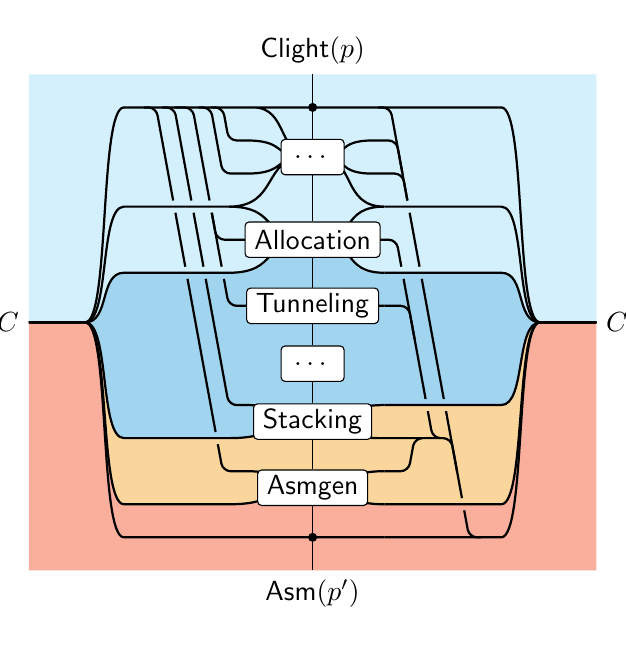
\begin{tikzpicture}[yscale=0.42,xscale=0.7]
    \tikzset{to path={
      .. controls ($(\tikztostart)!\stens!(\tikztostart -| \tikztotarget)$)
              and ($(\tikztotarget)!\stens!(\tikztotarget -| \tikztostart)$) ..
      (\tikztotarget) \tikztonodes}}

    % Refinement of the incoming convention
    \begin{scope}[xshift=1.3cm,xscale=0.11]

      % Fan out from here
      \coordinate (RB) at (27,7.5);
      \coordinate (R) at (35,7.5);

      \drawsc (-1,14) coordinate (XI1) -- (18,14) to (RB) -- (R);
      \drawsc (0,11) coordinate (AI1) -- (18,11) to (RB) -- (R);
      \drawsc (0, 9) coordinate (AI3) -- (18, 9) coordinate (CLI) to (RB) -- (R);
      \drawsc (0, 5) coordinate (SI1) -- (18, 5) coordinate (LMI) to (RB) -- (R);
      \drawsc (0, 2) coordinate (GI2) -- (18, 2) coordinate (MAI) to (RB) -- (R);
      \drawsc (0, 1) coordinate (RaI) -- (18, 1) to (RB) -- (R);
      \node[right,overlay] at (R) {$\mathbb{C}$};

      % From now on we will use nodes as gaps around crossings
      \tikzset{every node/.style={inner sep=2pt}};

      % The vainj across
      \node (C1) at (4,11) {};
      \node (C2) at (6, 9) {};
      \node (C3) at (10,5) {};
      \node (C4) at (13,2) {};
      \drawsc (XI1) -- (1,14) -- (C1) -- (C2) -- (C3) -- (C4) -- (14,1) -- (16,1);

      % Spikes off of vainj
      \drawsc (-2,13) coordinate (XI2) -- (2,13) -- (3,12); % inj
      \drawsc (-2,12) coordinate (XI3) -- (3,12) -- (C1); % vainj
      \drawsc (-1, 4) coordinate (SI2) -- (11,4) -- (12,3); % inj

      % Spikes off of that last inj
      \node (C5) at (3,9) {};
      \node (C6) at (7,5) {};
      \drawsc (-1,10) coordinate (AI2) -- (2,10) -- (C5) -- (C6) -- (8,4) -- (9,4); % ext
      \drawsc (0, 8) coordinate (TI) -- (4,8) -- (5,7); % ext
      \drawsc (0, 3) coordinate (GI1) -- (4,3) -- (5,4) -- (6,4); % ext
    \end{scope}

    % Refinement of the outgoing convention
    \begin{scope}[xshift=-1.52cm,xscale=-0.11]

      % Fan out from here
      \coordinate (LB) at (25,7.5);
      \coordinate (L) at (33,7.5);

      \drawsc (-4,14) coordinate (XO1) -- (16,14) to (LB) -- (L);
      \drawsc (0,11) coordinate (AO1) -- (16,11) to (LB) -- (L);
      \drawsc (0, 9) coordinate (AO3) -- (16, 9) coordinate (CLO) to (LB) -- (L);
      \drawsc (0, 4) coordinate (SO1) -- (16, 4) coordinate (LMO) to (LB) -- (L);
      \drawsc (0, 2) coordinate (GO2) -- (16, 2) coordinate (MAO) to (LB) -- (L);
      \drawsc (0, 1) coordinate (RaO) -- (16, 1) to (LB) -- (L);
      \node[left,overlay] at (L) {$\mathbb{C}$};

      % From now on we will use nodes as gaps around crossings
      \tikzset{every node/.style={inner sep=2pt}};

      % Asmgen
      \node (D1) at ( 2, 4) {};
      \node (D2) at ( 7, 9) {};
      \node (D3) at ( 9,11) {};
      \drawsc (-3, 3) coordinate (GO1) -- (1, 3) -- (D1) -- (D2) -- (D3) -- (12,14) -- (14,14);

      % Stacking
      \node (D5) at ( 4, 9) {};
      \node (D6) at ( 6,11) {};
      \drawsc (-3, 5) coordinate (SO2) -- (0, 5) -- (D5) -- (D6) -- (9,14) -- (11,14);

      % Tunneling
      \node (D7) at ( 1, 9) {};
      \node (D8) at ( 3,11) {};
      \drawsc (-3, 8) coordinate (TO)  -- (0, 8) -- (D7) -- (D8);

      % Allocation
      \drawsc (-3,10) coordinate (AO2) -- (2,10) -- (D8) -- ( 6,14) -- ( 9,14);

      % Frontend
      \drawsc (-3,12) coordinate (XO3) -- (1,12) -- ( 3,14) -- ( 5,14);
      \drawsc (-3,13) coordinate (XO2) -- (0,13) -- ( 1,14) -- ( 3,14);
    \end{scope}

    % Nodes
    \begin{scope}
      \begin{pgfonlayer}{nodes}
        \begin{scope}[every node/.style={draw,fill=white,rounded corners=0.5mm,minimum height=0.45cm,inner ysep=0pt}]
          \node[minimum width=0.8cm] (X) at (0,12.5) {\ldots};
          \node (A) at (0,10) {$\kw{Allocation}$};
          \node (T) at (0,8) {$\kw{Tunneling}$};
          \node[minimum width=0.8cm] (C) at (0,6.25) {\ldots};
          \node (S) at (0,4.5) {$\kw{Stacking}$};
          \node (G) at (0,2.5) {$\kw{Asmgen}$};
        \end{scope}
        \begin{scope}[every node/.style={fill=black,draw=black,circle,inner sep=1pt}]
          \node (RC) at (0,14) {};
          \node (RA) at (0,1) {};
        \end{scope}
      \end{pgfonlayer}
    \end{scope}

    \draw[thin]
      (0,15) coordinate (SP) node[above] {$\kw{Clight}(p)$} --
      (X) -- (A) -- (T) -- (C) -- (S) -- (G) -- (RA) --
      (0,0) coordinate (TP) node[below] {$\kw{Asm}(p')$};

    \drawsc
      (XI1) to (RC.center) to (XO1)
               (X.center) to (XO1)
      (XI2) to (X.center) to (XO2)
      (XI3) to (X.center) to (XO3)
      (AI1) to (X.center) to (AO1)
      (AI1) to (A.center) to (AO1)
      (AI2) to (A.center) to (AO2)
      (AI3) to (A.center) to (AO3)
      (TI)  to (T.center) to (TO)
      (SI1) to (S.center) to (SO1)
      (SI2) to (S.center) to (SO2)
      (GI1) to (G.center) to (GO1)
      (GI2) to (G.center) to (GO2)
      (RaI) to (RA.center) to (RaO);

    % Extra simulation convention labels
%    \tiny
%    \path[every node/.style={inner sep=0.8pt}]
%      (XI2) node[above] {$\kw{inj}$}
%      (XI3) node[above] {$\kw{vainj}$}
%      (GI1) node[above] {$\kw{ext}$}
%      (SI2) node[above] {$\kw{inj}$}
%      (TI)  node[above] {$\kw{ext}$}
%      (AI2) node[above] {$\kw{ext}$}
%      (XO2) node[above] {$\kw{inj}$}
%      (XO3) node[above] {$\kw{vainj}$}
%      (AO2) node[above] {$\kw{ext}$}
%      (TO) node[above] {$\kw{ext}$}
%      (SO2) node[above] {$\kw{injp}$}
%      (GO1) node[above] {$\kw{ext}$};

    % Region coloring
    \begin{pgfonlayer}{tint}
      \fill[ACMLightBlue\filltint]
        (R) [rounded corners=1mm] -- (RB) to (CLI) --
        (AI3) to (A.center) to (AO3) --
        (CLO) to (LB) [rounded corners=0] -- (L) |- (SP) -| cycle;
      \fill[ACMBlue\filltint,rounded corners=1mm]
        (RB) to
        (CLI) -- (AI3) to (A.center) to (AO3) -- (CLO) to (LB) to
        (LMO) -- (SO1) to (S.center) to (SI1) -- (LMI) to cycle;
      \fill[ACMOrange\filltint, rounded corners=1mm]
        (L) -- (LB) to
        (LMO) -- (SO1) to (S.center) to (SI1) -- (LMI) to (RB) to
        (MAI) -- (GI2) to (G.center) to (GO2) -- (MAO) to (LB) -- cycle;
      \fill[ACMRed\filltint]
        (R) [rounded corners=1mm] -- (RB) to
        (MAI) -- (GI2) to (G.center) to (GO2) -- (MAO) to (LB) [rounded corners=0] --
        (L) |- (TP) -| cycle;
    \end{pgfonlayer}
  \end{tikzpicture}
  %}}}
  \end{columns}
\end{frame}
%}}}

\begin{frame}{CompCertO uses three kinds of simulation conventions} %{{{
  \begin{itemize}
    \item Proper \textbf{calling conventions} across different language interfaces
      \[
        \begin{tile}{}
          \filltop{ACMLightBlue\filltint}
          \fillbot{ACMBlue\filltint}
          \drawsc (L) -- (R)
            node[right] {$\cc{C}{L} : \mathcal{C} \Leftrightarrow \mathcal{L}$};
        \end{tile}
        \qquad
        \begin{tile}{}
          \filltop{ACMBlue\filltint}
          \fillbot{ACMOrange\filltint}
          \drawsc (L) -- (R)
            node[right] {$\cc{L}{M} : \mathcal{L} \Leftrightarrow \mathcal{M}$};
        \end{tile}
        \qquad
        \begin{tile}{}
          \filltop{ACMOrange\filltint}
          \fillbot{ACMRed\filltint}
          \drawsc (L) -- (R)
            node[right] {$\cc{M}{A} : \mathcal{M} \Leftrightarrow \mathcal{A}$};
        \end{tile}
      \]
    \pause
    \item CompCert \textbf{Kripke logical relations} to capture memory transformations
      \[
        \mathbf{R} \in \{ \kw{ext}\,, \kw{inj}\,, \kw{injp}\,, \kw{vaext}\,, \kw{vainj} \}
        \qquad
        \mathbf{R}_\mathcal{X} : \mathcal{X} \Leftrightarrow \mathcal{X}
      \]
      \[
        \begin{tile}{}
          \fillboth{ACMLightBlue\filltint}
          \drawsc (L) -- (R) node[right] {$\mathbf{R}_\mathcal{C}$};
        \end{tile}
        \qquad
        \begin{tile}{}
          \fillboth{ACMBlue\filltint}
          \drawsc (L) -- (R) node[right] {$\mathbf{R}_\mathcal{L}$};
        \end{tile}
        \qquad
        \begin{tile}{}
          \fillboth{ACMOrange\filltint}
          \drawsc (L) -- (R) node[right] {$\mathbf{R}_\mathcal{M}$};
        \end{tile}
        \qquad
        \begin{tile}{}
          \fillboth{ACMRed\filltint}
          \drawsc (L) -- (R) node[right] {$\mathbf{R}_\mathcal{A}$};
        \end{tile}
      \]
    \pause
    \item \textbf{Invariants} to impose typing and other constraints
      on questions and answers
      \[
        \begin{tile}{}
          \fillboth{ACMLightBlue\filltint}
          \drawsc (L) -- (R)
            node[right] {$\kw{wt} : \mathcal{C} \Leftrightarrow \mathcal{C}$};
        \end{tile}
        \qquad
        \begin{tile}{}
          \fillboth{ACMLightBlue\filltint}
          \drawsc (L) -- (R)
            node[right] {$\kw{va} : \mathcal{C} \Leftrightarrow \mathcal{C}$};
        \end{tile}
      \]
  \end{itemize}
\end{frame}
%}}}

\begin{frame}{Some Refinement Properties used in CompCertO} %{{{
  \begin{itemize}
    \item CompCert KLRs compose in various ways
    \[
      \begin{tile}{}
        \fillboth{ACMLightBlue\filltint}
        \drawsc (BL) node[left] {$\kw{inj}$} -- (BLB) -- (C.center) -- (R) node[right] {$\kw{inj}$};
        \drawsc (TL) node[left] {$\kw{ext}$} -- (TLB) -- (C.center) -- (R);
      \end{tile}
      \qquad
      \begin{tile}{}
        \fillboth{ACMLightBlue\filltint}
        \drawsc (L) node[left] {$\kw{inj}$} -- (C.center) -- (BRB) -- (BR) node[right] {$\kw{ext}$};
        \drawsc (L) -- (C.center) -- (TRB) -- (TR) node[right] {$\kw{inj}$};
      \end{tile}
    \]
    \pause
    \item Calling conventions and invariants commute with KLRs
    \[
      \begin{tile}{}
        \drawsc (L) node[left] {$\cc{X}{Y}$}
          -- (R) node[right] {$\cc{X}{Y}$};
        \drawsc (TL) node[left] {$\mathbf{R}$}
          -- (TLB) -- (C) -- (BRB)
          -- (BR) node[right] {$\mathbf{R}$};
        \filltop{ACMOrange\filltint}
        \fillbot{ACMRed\filltint}
        \node[below left,inner sep=1pt] at (TRC) {\tiny $\mathcal{X}$};
        \node[above right,inner sep=1pt] at (BLC) {\tiny $\mathcal{Y}$};
      \end{tile}
      \qquad \quad
      \begin{tile}{}
        \drawsc (L) node[left] {$\mathbb{R}$} -- (C) -- (R) node[right] {$\mathbb{R}$};
        \drawsc (BL) node[left] {$\kw{wt}$} -- (BR) node[right] {$\kw{wt}$};
        \drawsc (BL) -- (BLB) -- (TRB) -- (TR) node[right] {$\kw{wt}$};
        \fillboth{ACMLightBlue\filltint}
      \end{tile}
      \quad
      \begin{tile}{}
        \drawsc (L) node[left] {$\mathbb{R}$} -- (C) -- (R) node[right] {$\mathbb{R}$};
        \drawsc (BL) node[left] {$\kw{wt}$} -- (BR) node[right] {$\kw{wt}$};
        \drawsc (TL) node[left] {$\kw{wt}$} -- (TLB) -- (BRB) -- (BR);
        \fillboth{ACMLightBlue\filltint}
      \end{tile}
      \quad
      \begin{tile}{}
        \drawsc (L) node[left] {$\kw{wt}$} -- (R) node[right] {$\kw{wt}$};
        \drawsc (TL) node[left] {$\mathbb{R}$} -- (TLB) -- (C) -- (BRB) -- (BR) node[right] {$\mathbb{R}$};
        \fillboth{ACMLightBlue\filltint}
      \end{tile}
    \]
    \pause
    \item Simulation conventions carry a typed Kleene algebra
  \end{itemize}
\end{frame}
%}}}

\begin{frame}{Structure of the Correctness Proof} %{{{
  \centering
  \figsize
  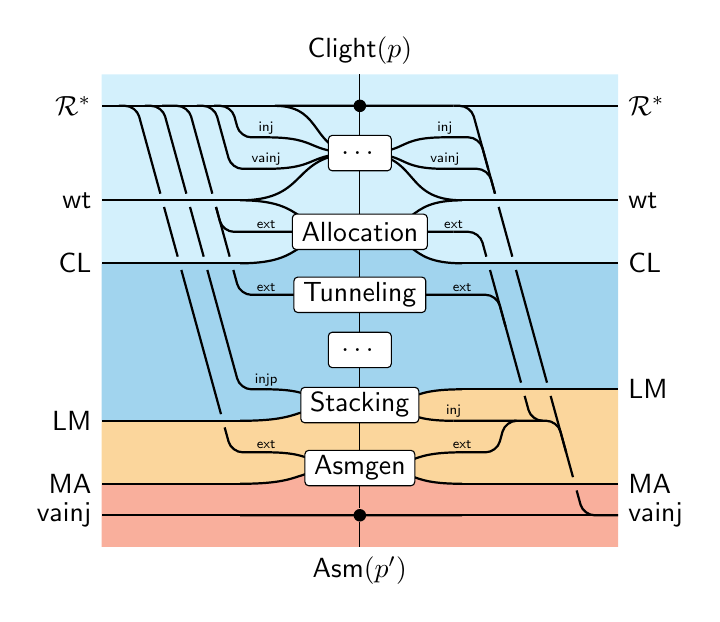
\begin{tikzpicture}[yscale=0.4,thick]
    \tikzset{to path={
      .. controls ($(\tikztostart)!\stens!(\tikztostart -| \tikztotarget)$)
              and ($(\tikztotarget)!\stens!(\tikztotarget -| \tikztostart)$) ..
      (\tikztotarget) \tikztonodes}}

    % Refinement of the incoming convention
    \begin{scope}[xshift=1.3cm,xscale=0.11]
      \draw (-1,14) coordinate (XI1) -- (18,14) node[right] {$\mathcal{R}^*$};
      \draw (0,11) coordinate (AI1) -- (18,11) node[right] {$\kw{wt}$};
      \draw (0, 9) coordinate (AI3) -- (18, 9) coordinate (CLI) node[right] {$\cc{C}{L}$};
      \draw (0, 5) coordinate (SI1) -- (18, 5) coordinate (LMI) node[right] {$\cc{L}{M}$};
      \draw (0, 2) coordinate (GI2) -- (18, 2) coordinate (MAI) node[right] {$\cc{M}{A}$};
      \draw (0, 1) coordinate (RaI) -- (18, 1) node[right] {$\kw{vainj}$};

      % From now on we will use nodes as gaps around crossings
      \tikzset{rounded corners,every node/.style={inner sep=2pt}};

      % The vainj across
      \node (C1) at (4,11) {};
      \node (C2) at (6, 9) {};
      \node (C3) at (10,5) {};
      \node (C4) at (13,2) {};
      \draw (XI1) -- (1,14) -- (C1) -- (C2) -- (C3) -- (C4) -- (14,1) -- (18,1);

      % Spikes off of vainj
      \draw (-2,13) coordinate (XI2) -- (2,13) -- (3,12); % inj
      \draw (-2,12) coordinate (XI3) -- (3,12) -- (C1); % vainj
      \draw (-1, 4) coordinate (SI2) -- (11,4) -- (12,3); % inj

      % Spikes off of that last inj
      \node (C5) at (3,9) {};
      \node (C6) at (7,5) {};
      \draw (-1,10) coordinate (AI2) -- (2,10) -- (C5) -- (C6) -- (8,4) -- (9,4); % ext
      \draw (0, 8) coordinate (TI) -- (4,8) -- (5,7); % ext
      \draw (0, 3) coordinate (GI1) -- (4,3) -- (5,4) -- (6,4); % ext
    \end{scope}

    % Refinement of the outgoing convention
    \begin{scope}[xshift=-1.52cm,xscale=-0.11]
      \draw (-4,14) coordinate (XO1) -- (16,14) node[left] {$\mathcal{R}^*$};
      \draw (0,11) coordinate (AO1) -- (16,11) node[left] {$\kw{wt}$};
      \draw (0, 9) coordinate (AO3) -- (16, 9) coordinate (CLO) node[left] {$\cc{C}{L}$};
      \draw (0, 4) coordinate (SO1) -- (16, 4) coordinate (LMO) node[left] {$\cc{L}{M}$};
      \draw (0, 2) coordinate (GO2) -- (16, 2) coordinate (MAO) node[left] {$\cc{M}{A}$};
      \draw (0, 1) coordinate (RaO) -- (16, 1) node[left] {$\kw{vainj}$};

      % From now on we will use nodes as gaps around crossings
      \tikzset{rounded corners,every node/.style={inner sep=2pt}};

      % Asmgen
      \node (D1) at ( 2, 4) {};
      \node (D2) at ( 7, 9) {};
      \node (D3) at ( 9,11) {};
      \draw (-3, 3) coordinate (GO1) -- (1, 3) -- (D1) -- (D2) -- (D3) -- (12,14) -- (14,14);

      % Stacking
      \node (D5) at ( 4, 9) {};
      \node (D6) at ( 6,11) {};
      \draw (-3, 5) coordinate (SO2) -- (0, 5) -- (D5) -- (D6) -- (9,14) -- (11,14);

      % Tunneling
      \node (D7) at ( 1, 9) {};
      \node (D8) at ( 3,11) {};
      \draw (-3, 8) coordinate (TO)  -- (0, 8) -- (D7) -- (D8);

      % Allocation
      \draw (-3,10) coordinate (AO2) -- (2,10) -- (D8) -- ( 6,14) -- ( 9,14);

      % Frontend
      \draw (-3,12) coordinate (XO3) -- (1,12) -- ( 3,14) -- ( 5,14);
      \draw (-3,13) coordinate (XO2) -- (0,13) -- ( 1,14) -- ( 3,14);
    \end{scope}

    % Nodes
    \begin{scope}
      \begin{pgfonlayer}{nodes}
        \begin{scope}[every node/.style={draw,fill=white,rounded corners=0.5mm,minimum height=0.45cm,inner ysep=0pt}]
          \node[minimum width=0.8cm] (X) at (0,12.5) {\ldots};
          \node (A) at (0,10) {$\kw{Allocation}$};
          \node (T) at (0,8) {$\kw{Tunneling}$};
          \node[minimum width=0.8cm] (C) at (0,6.25) {\ldots};
          \node (S) at (0,4.5) {$\kw{Stacking}$};
          \node (G) at (0,2.5) {$\kw{Asmgen}$};
        \end{scope}
        \begin{scope}[every node/.style={fill=black,circle,inner sep=1.6pt}]
          \node (RC) at (0,14) {};
          \node (RA) at (0,1) {};
        \end{scope}
      \end{pgfonlayer}
    \end{scope}

    \draw[thin]
      (0,15) coordinate (SP) node[above] {$\kw{Clight}(p)$} --
      (X) -- (A) -- (T) -- (C) -- (S) -- (G) -- (RA) --
      (0,0) coordinate (TP) node[below] {$\kw{Asm}(p')$};

    \draw
      (XI1) to (RC.center) to (XO1)
               (X.center) to (XO1)
      (XI2) to (X.center) to (XO2)
      (XI3) to (X.center) to (XO3)
      (AI1) to (X.center) to (AO1)
      (AI1) to (A.center) to (AO1)
      (AI2) to (A.center) to (AO2)
      (AI3) to (A.center) to (AO3)
      (TI)  to (T.center) to (TO)
      (SI1) to (S.center) to (SO1)
      (SI2) to (S.center) to (SO2)
      (GI1) to (G.center) to (GO1)
      (GI2) to (G.center) to (GO2)
      (RaI) to (RA.center) to (RaO);

    % Extra simulation convention labels
    \tiny
    \path[every node/.style={inner sep=0.8pt}]
      (XI2) node[above] {$\kw{inj}$}
      (XI3) node[above] {$\kw{vainj}$}
      (GI1) node[above] {$\kw{ext}$}
      (SI2) node[above] {$\kw{inj}$}
      (TI)  node[above] {$\kw{ext}$}
      (AI2) node[above] {$\kw{ext}$}
      (XO2) node[above] {$\kw{inj}$}
      (XO3) node[above] {$\kw{vainj}$}
      (AO2) node[above] {$\kw{ext}$}
      (TO) node[above] {$\kw{ext}$}
      (SO2) node[above] {$\kw{injp}$}
      (GO1) node[above] {$\kw{ext}$};

    % Region coloring
    \begin{pgfonlayer}{tint}
      \fill[ACMLightBlue\filltint]
        (AI3) to (A.center) to (AO3) --
        (CLO) |- (SP) -| (CLI) -- cycle;
      \fill[ACMBlue\filltint]
        (CLI) -- (AI3) to (A.center) to (AO3) -- (CLO) --
        (LMO) -- (SO1) to (S.center) to (SI1) -- (LMI) -- cycle;
      \fill[ACMOrange\filltint]
        (LMO) -- (SO1) to (S.center) to (SI1) -- (LMI) --
        (MAI) -- (GI2) to (G.center) to (GO2) -- (MAO) -- cycle;
      \fill[ACMRed\filltint]
        (MAI) -- (GI2) to (G.center) to (GO2) -- (MAO) |- (TP) -| cycle;
    \end{pgfonlayer}

  \end{tikzpicture}
\end{frame}
%}}}

\section*{Conclusion}

\begin{frame}{Conclusion}
CompCertO achieves full compositionality through:
\begin{itemize}
  \item Open semantics with coarse-grained types
  \item Flexible treatment of simulation conventions
  \item Simulation convention algebra
\end{itemize}
Our model can be embedded into richer ones
for heterogeneous verification.

\pause\vfill
The full development is available online:
\begin{itemize}
  \item Source code: \url{https://github.com/CertiKOS/compcert/tree/compcerto}
  \item Documentation: \url{https://certikos.github.io/compcert/}
\end{itemize}
\end{frame}

\begin{frame}
  \centering
  \Large
  Thank you for watching!
\end{frame}

\end{document}
